% !TeX root = ../main.tex
% Add the above to each chapter to make compiling the PDF easier in some editors.

\chapter{Datasets}\label{chapter:datasets}
We evaluate the efficiency and performance of combinations of active learning algorithms, pre-training methods, and training strategies on three fully annotated datasets from the biomedical imaging field (Figure \ref{fig:datasets_composition}).

\begin{figure}[htbp]
\centering
\captionsetup{format=plain}
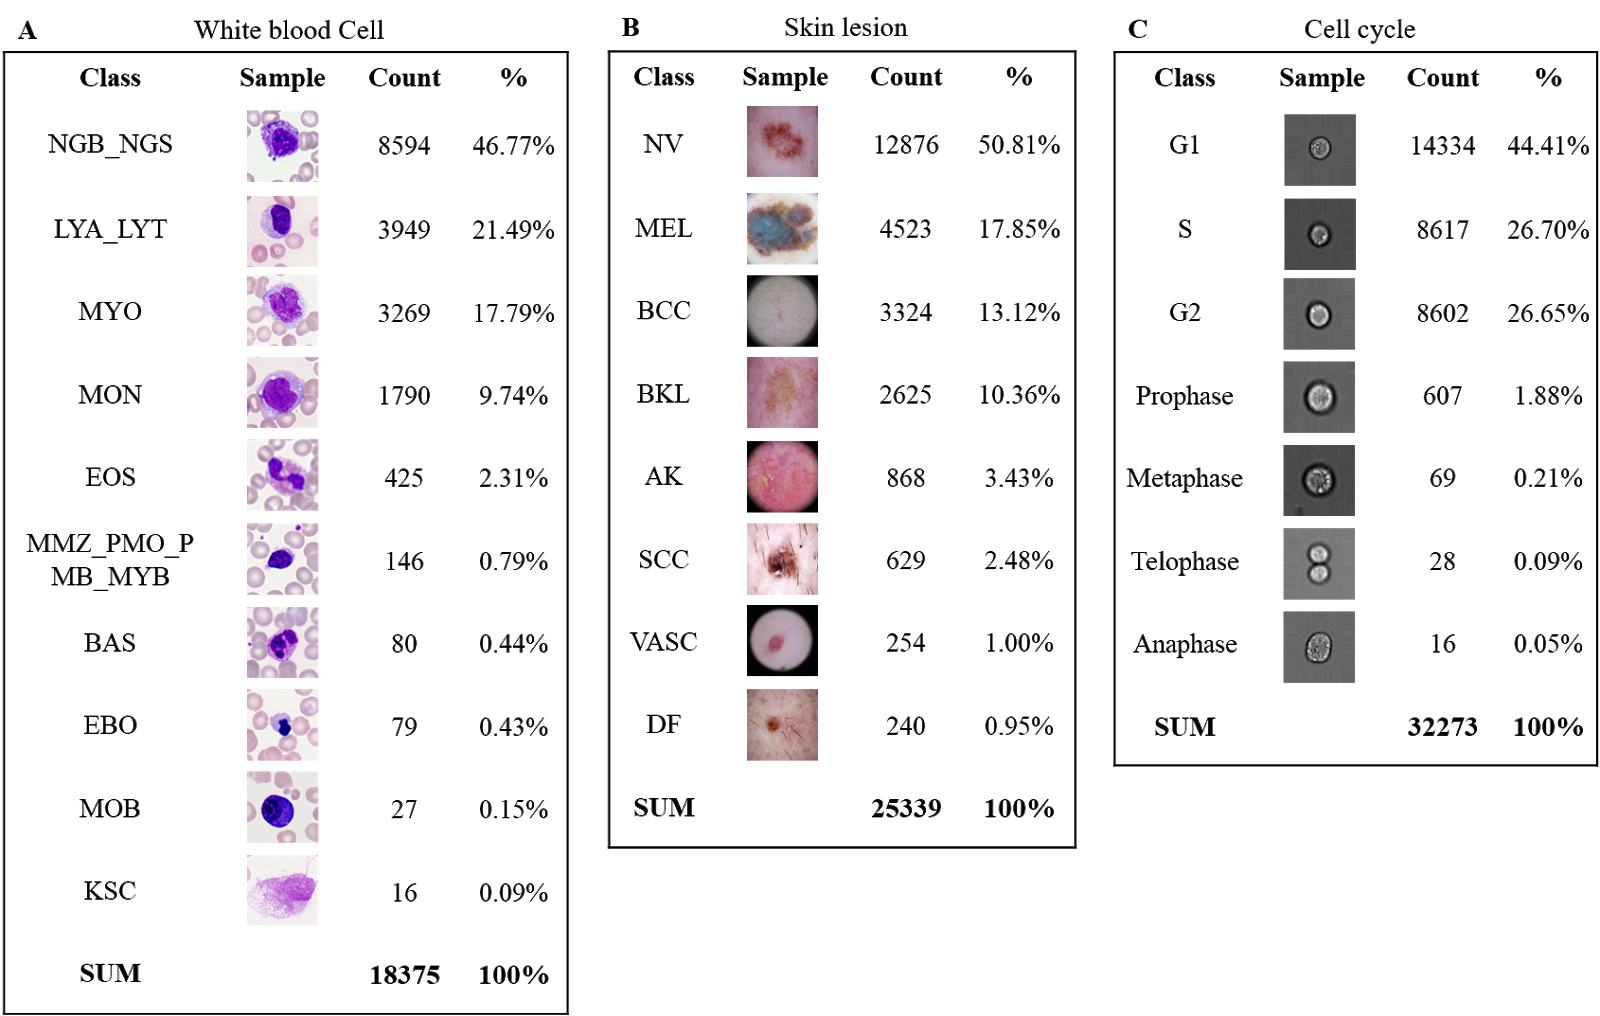
\includegraphics[width=0.95\textwidth]{figures/fig_datasets_composition.png}
\caption{Biomedical image datasets used in this study are exhibiting strong class imbalance, little color variance and high similarity between classes. (A) White blood cell: A dataset with 18357 images (128x128 pixel) of white human blood cells with ten expert labeled classes from blood smears of 100 patients diagnosed with Acute Myeloid Leukemia (AML) and 100 individuals which show no symptoms of the disease \cite{matek2019, clark2013}. (B) Skin lesion: A dataset with 25339 dermoscopy images (128x128 pixel) of skin lesions with eight skin cancer classes \cite{codella2018, combalia2019, tschandl2018}. (C) Cell cycle: A dataset comprising 32272 images (64x64 pixel) of Jurkat cells in seven different cell cycle stages created by imaging flow cytometry \cite{eulenberg2017}.}
\label{fig:datasets_composition}
\end{figure}

\newpage

% rework these sections to make them different from what it says on their websites
\section{White Blood Cells}

The Munich AML Morphology Dataset contains 18,365 expert-labeled single-cell images taken from peripheral blood smears of 100 patients diagnosed with Acute Myeloid Leukemia at Munich University Hospital between 2014 and 2017, as well as 100 patients without signs of hematological malignancy. Image acquisition was done using a M8 digital microscope / scanner (Precipoint GmbH, Freising, Germany) at 100-fold optical magnification and oil immersion. Pathological and non-pathological leukocytes were classified into a standard morphological classification scheme derived from clinical practice by trained experts. To quantify inter- and intra-rater variability of examiners, a subset of images was re-annotated up to two times. The dataset has been used by the authors to train a convolutional neural network for single-cell morphology classification.

\section{Skin Lesion}

The International Skin Imaging Collaboration: Melanoma Project is an academia and industry partnership designed to facilitate the application of digital skin imaging to help reduce melanoma mortality. When recognized and treated in its earliest stages, melanoma is readily curable. Digital images of skin lesions can be used to educate professionals and the public in melanoma recognition as well as directly aid in the diagnosis of melanoma through teledermatology, clinical decision support, and automated diagnosis. Currently, a lack of standards for dermatologic imaging undermines the quality and usefulness of skin lesion imaging. ISIC is developing proposed standards to address the technologies, techniques, and terminology used in skin imaging with special attention to the issues of privacy and interoperability (i.e., the ability to share images across technology and clinical platforms). In addition, ISIC has developed and is expanding an open source public access archive of skin images to test and validate the proposed standards. This archive serves as a public resource of images for teaching and for the development and testing of automated diagnostic systems

\section{Cell Cycle}

Images of 32,266 asynchronously growing Jurkat cells were captured with the ImageStream platform. The cells were fixed and stained with PI (propidium iodide) to quantify DNA content and a MPM2 (mitotic protein monoclonal) antibody to identify mitotic cells.